\documentclass{article}

\usepackage{amsmath}
\usepackage{graphicx}

\title{TEK5600 - Mandatory assignment}
\author{Iver Oknes}

\begin{document}
\maketitle

\section{Introduction}
This report the mandatory assignment for TEK5600 for the spring semester of 2025.
In this report implementations of geometric field lines and line integral convolution
are discussed. Implementations as well as the tunable parameters are talked about
and compared, followed by a short discussion of the future work that could be done
with this material.

\section{Field lines}
A classic way to visualise the flow of a vector field at a single point in time is the field line.
A field line is a the line that follows the flow such that the tangent of the line is the vector field.
This also represents the path a massless particle would flow in the field at that moment in time.
Mathematically, the field line is described as
$$ \frac{d \vec{x}}{ds} \times \vec{u}(\vec{x}) = \vec{0} $$
meaning the tangent of the parametric representation of the field line $\vec{x}$ is parallel to the
vector field evaluated at the field line $\vec{u}(\vec{x})$.

To create the field lines from a discrete vector field, a numeric integrator is used. The accuracy
of the field lines will depend on the type of numeric integrator used, as well as on the step size
used when integrating. The function used to generate each individual field line take as arguments
the vector field, a starting point, a line length, a maximum number of steps to avoid overlong
calculations, as well as which integrator to use, and wether to integrate the line backwards as well
as forwards.

\subsection{Integrators}
The two integrators for generating field lines that have been implemented and tested are the classic
Forward Euler method, which simply iterates by setting the next point to be
$\vec{p}_{i+1} = p_i + dx \vec{u}(\vec{p}_i)$
where $\vec{p}_i$ is the current point, and $\vec{u}$ is the vector field.

The second integrator used is the $4$th-order Runge Kutta methods, which uses a 4 step calculation
to iterate the value. It goes as follows:
$K_1 = dx \vec{u}(\vec{p}_i)$
$K_2 = dx \vec{u}(\vec{p}_{i} + 0.5 K_1)$
$K_3 = dx \vec{u}(\vec{p}_{i} + 0.5 K_2)$
$K_4 = dx \vec{u}(\vec{p}_{i} + K_3)$
$\vec{p}_{i+1} = p_i + \frac{1}{6} (K_1 + 2K_2 + 2K_3 + K_4)$

\subsection{Seeding strategies}
The two main seeding strategies implemented as pure seed point generation are uniform and random. The
uniform seeding strategy generates a uniform grid of points from which to draw the field lines.
The other strategy implemented is a random sampling of seeding points, done by simply drawing random
$x$ and $y$ coordinates.

The third seeding strategy used is a flow feature based strategy using a derived property
of the field, namely the vorticity, or curl, of the vector field. Randomly generating
seed points for the field lines with a probability based on the magnitude of the
vorticity

\subsection{Comparison}

It is clear the three seeding strategies give rather different results. Random
is obviously quite unpredictable, having the start points be wherever in the field.
This does give a good representation for high enough values of starting points,
but not necessarily in an effective way, since more points will create a more
cluttered image. With some tuning of the number of points and some luck in where
they are generated, good images can be obtained form this method however.

Uniform is a lot more predictable, but may suffer from a lack of detail in areas
of exceptionally fast or curved flow, as the even spacing of the lines starting
point may leave some areas of interest as blind spots. Clutter is less of a problem
since the starting points are more spaced out, but may still occur if the field
has sinks where many of the lines from different starting points will end up, like
is visible in the Isabel data.

An approach that combines the two ideas is using flow feature based seeding. This
creates random points, but with some guidance as to where the random points will
be placed. The implementation shown here uses absolute value of the vorticity of
the field as a distribution function for drawing points randomly. This means areas
of high curvature will have more field lines starting there, guaranteeing that
the features with high curvature will be shown given a high enough number of samples,
even for rather short field lines.

The vorticity based seeding seems to be a good mix of uniform and random seedings
benefits, creating a clear picture of the flow with a minimal amount of clutter.
More work with tuning the length of the field lines, as well as the number of
seed points could of course give an even clearer picture, but the example shown here
gives a clear idea of its advantages.

Another method that could be combined with either of the strategies used here is
a density based approach, limiting how densely the field lines are allowed to be
drawn to each other. Variants of this using offsets from already drawn field lines
to seed new field also seem to yield good results that eliminate clutter quite well.

\begin{figure}
\makebox[\textwidth][c]{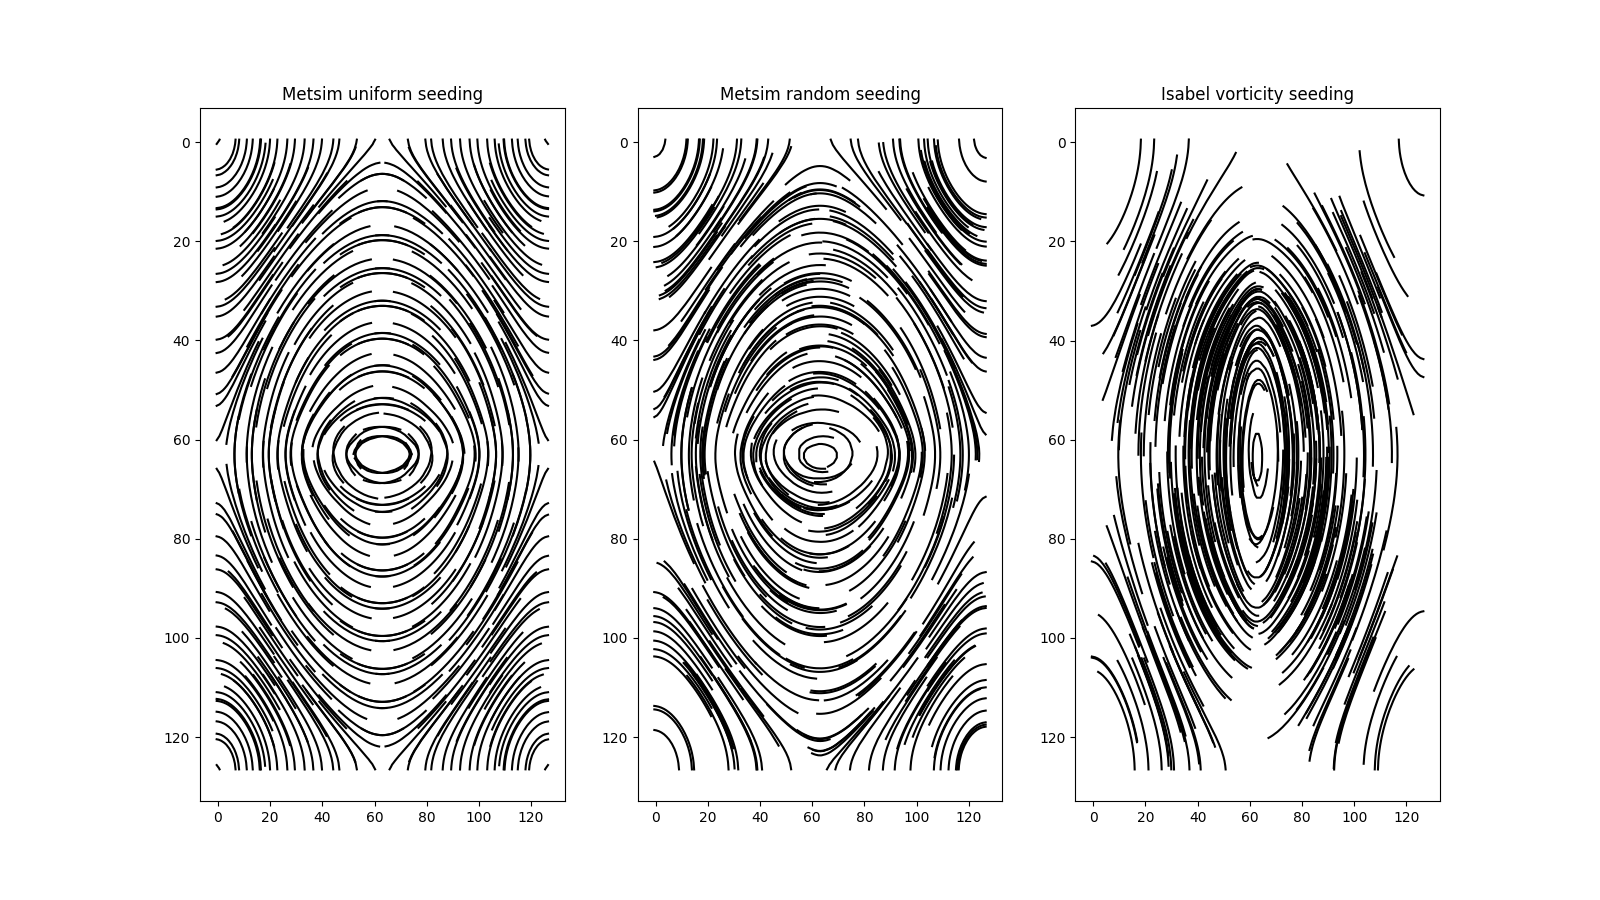
\includegraphics[width=18cm]{../output/metsim_seeding}}
\caption{Comparison of seeding strategies on the Metsim data}
\end{figure}

\begin{figure}
\makebox[\textwidth][c]{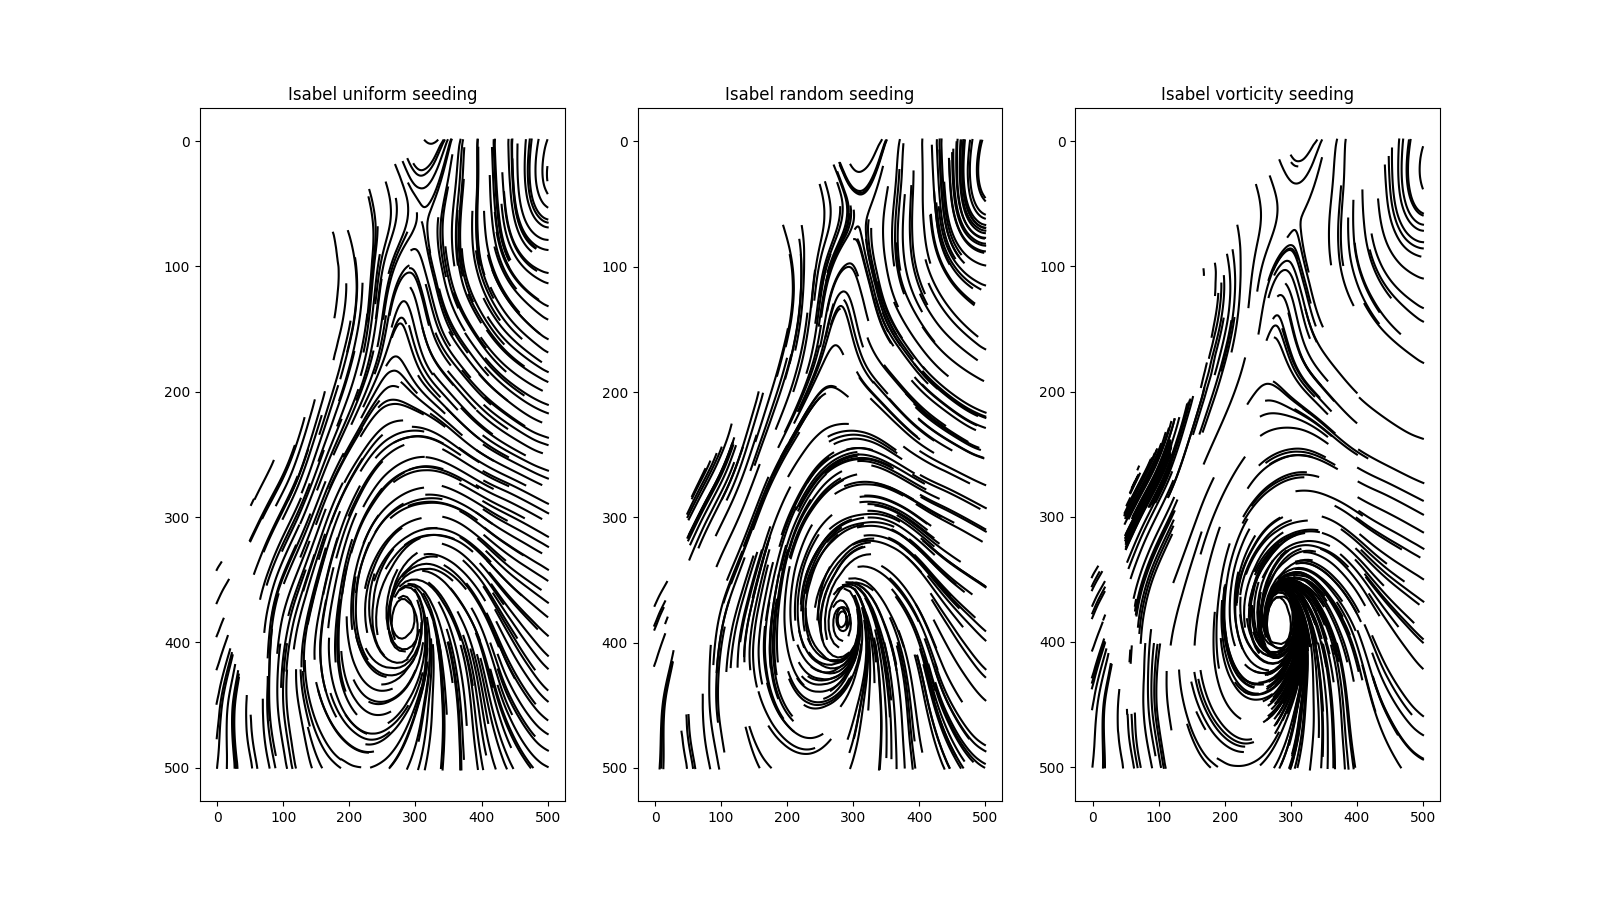
\includegraphics[width=18cm]{../output/isabel_seeding}}
\caption{Comparison of seeding strategies on the Isabel data}
\end{figure}

\begin{figure}
\makebox[\textwidth][c]{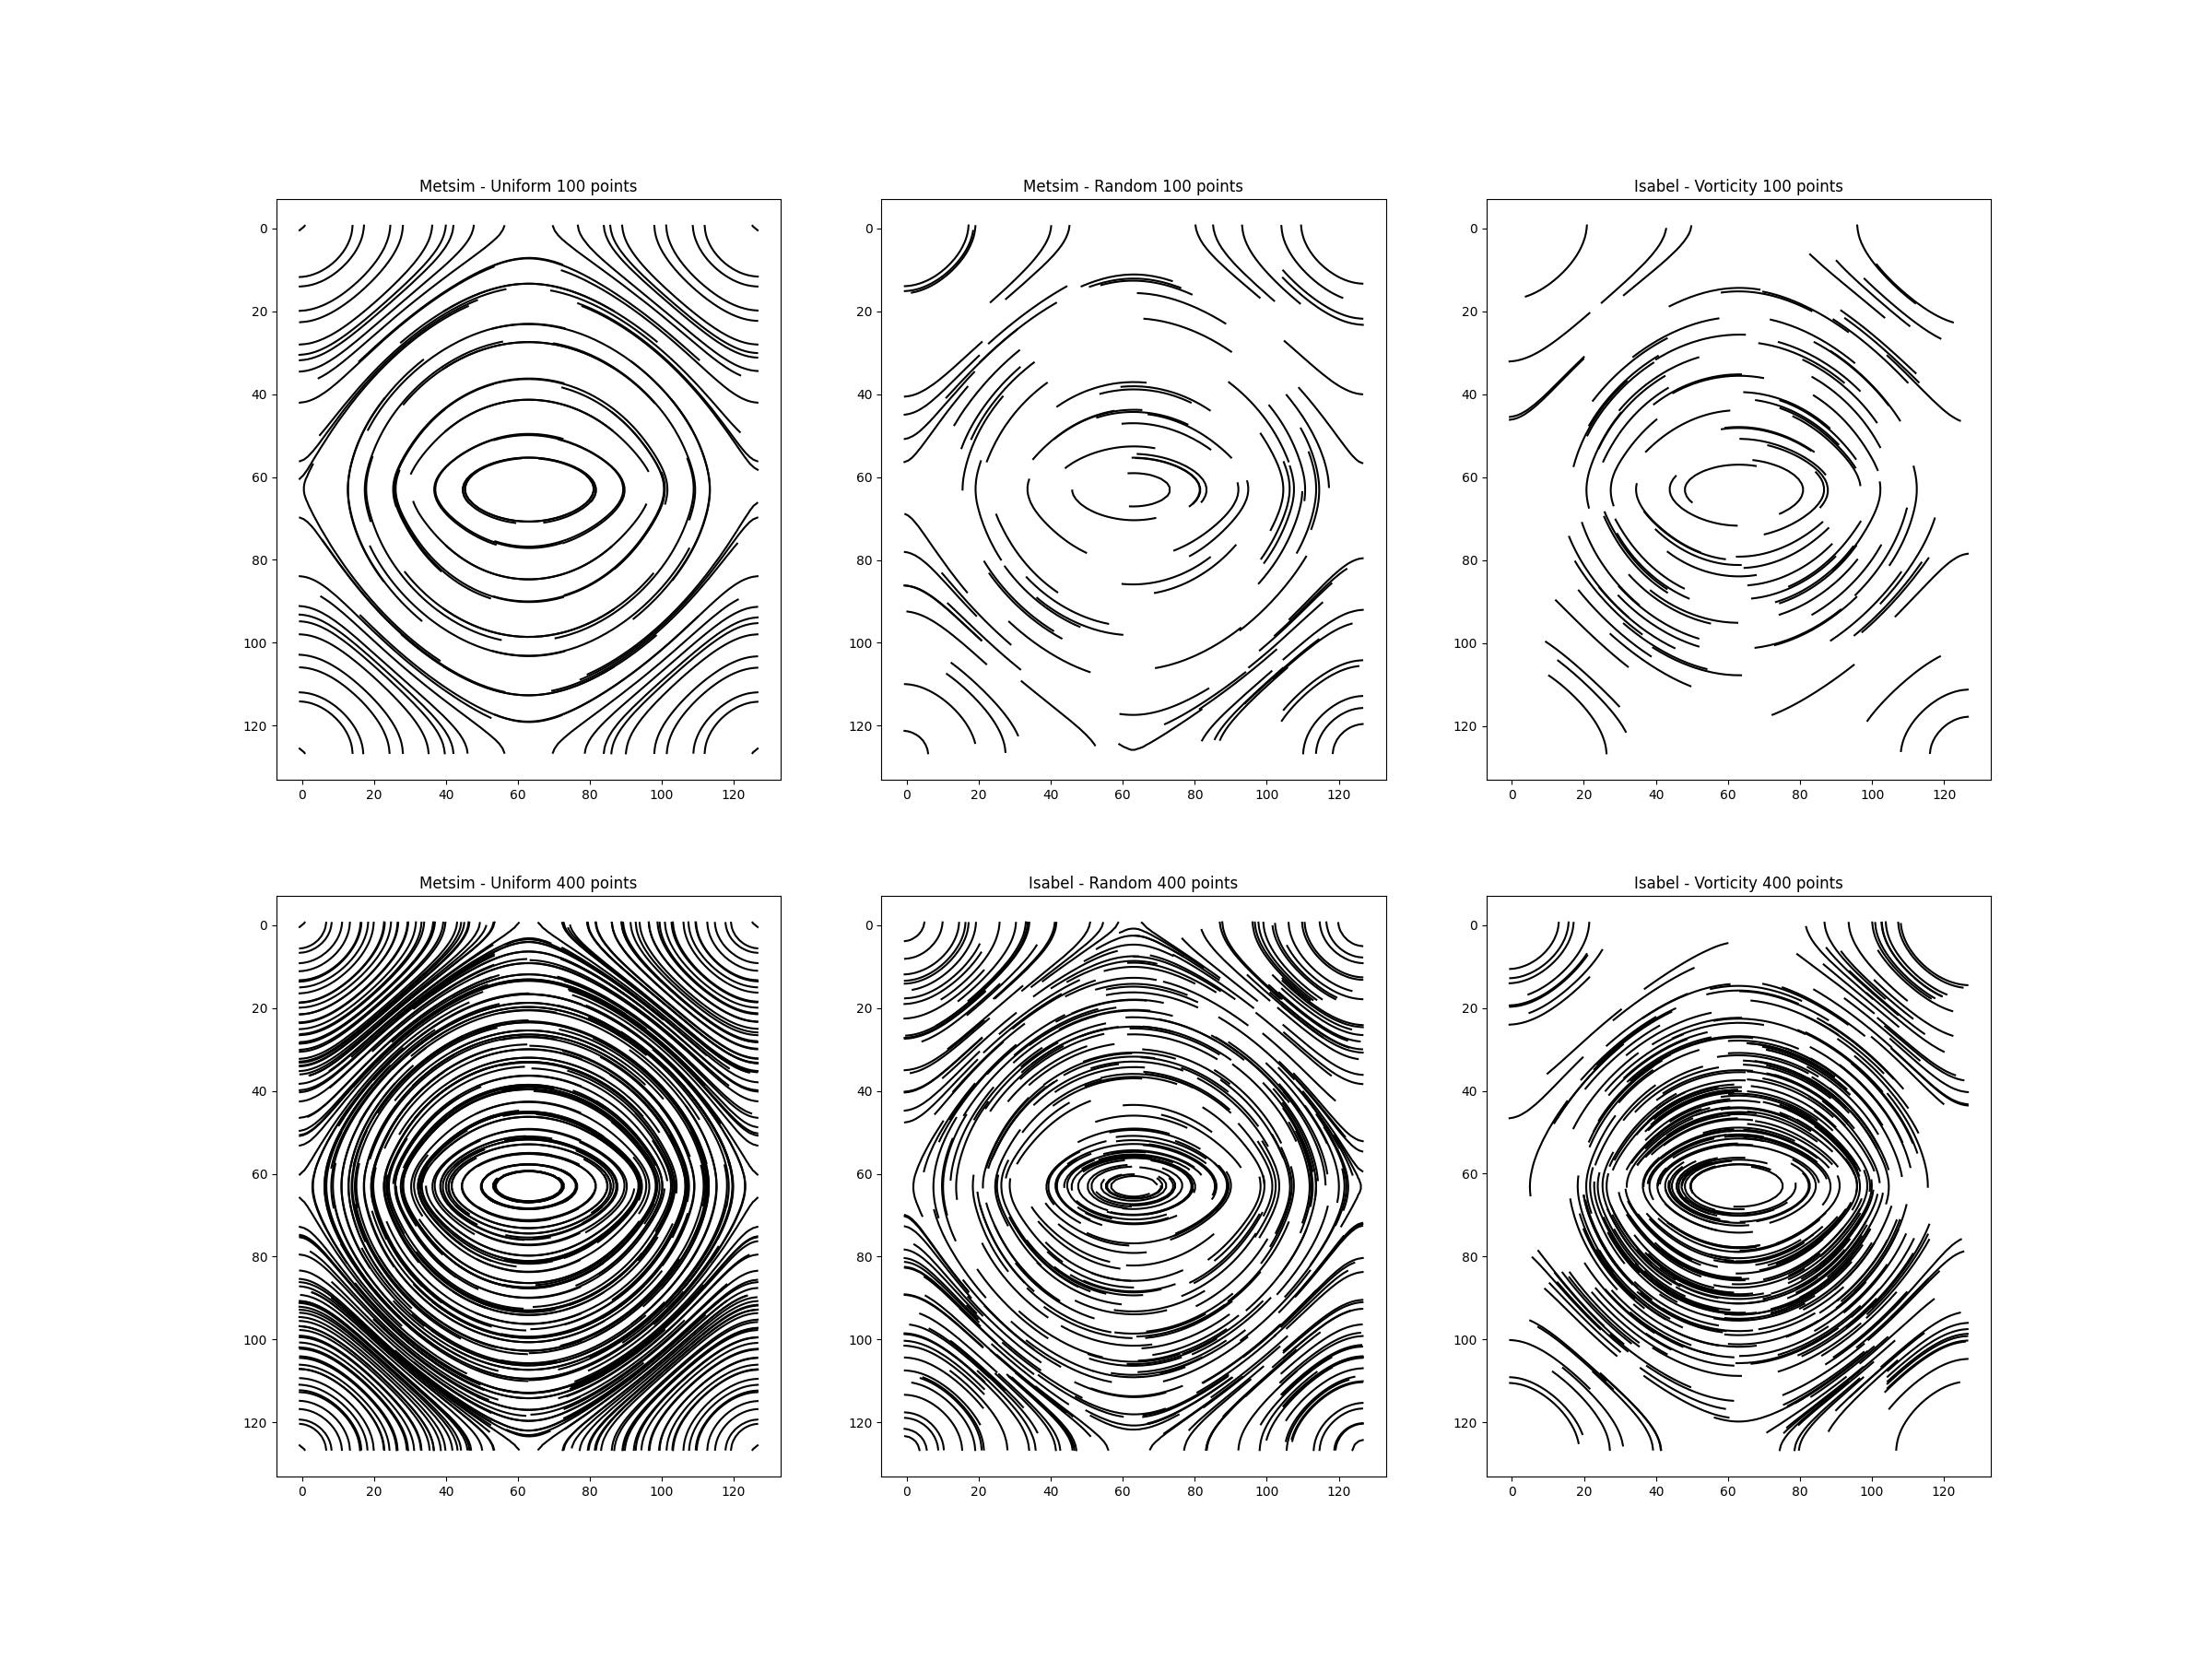
\includegraphics[width=18cm]{../output/metsim_seed_density.png}}
\caption{Comparison of seeding densities on the Metsim data}
\end{figure}

\begin{figure}
\makebox[\textwidth][c]{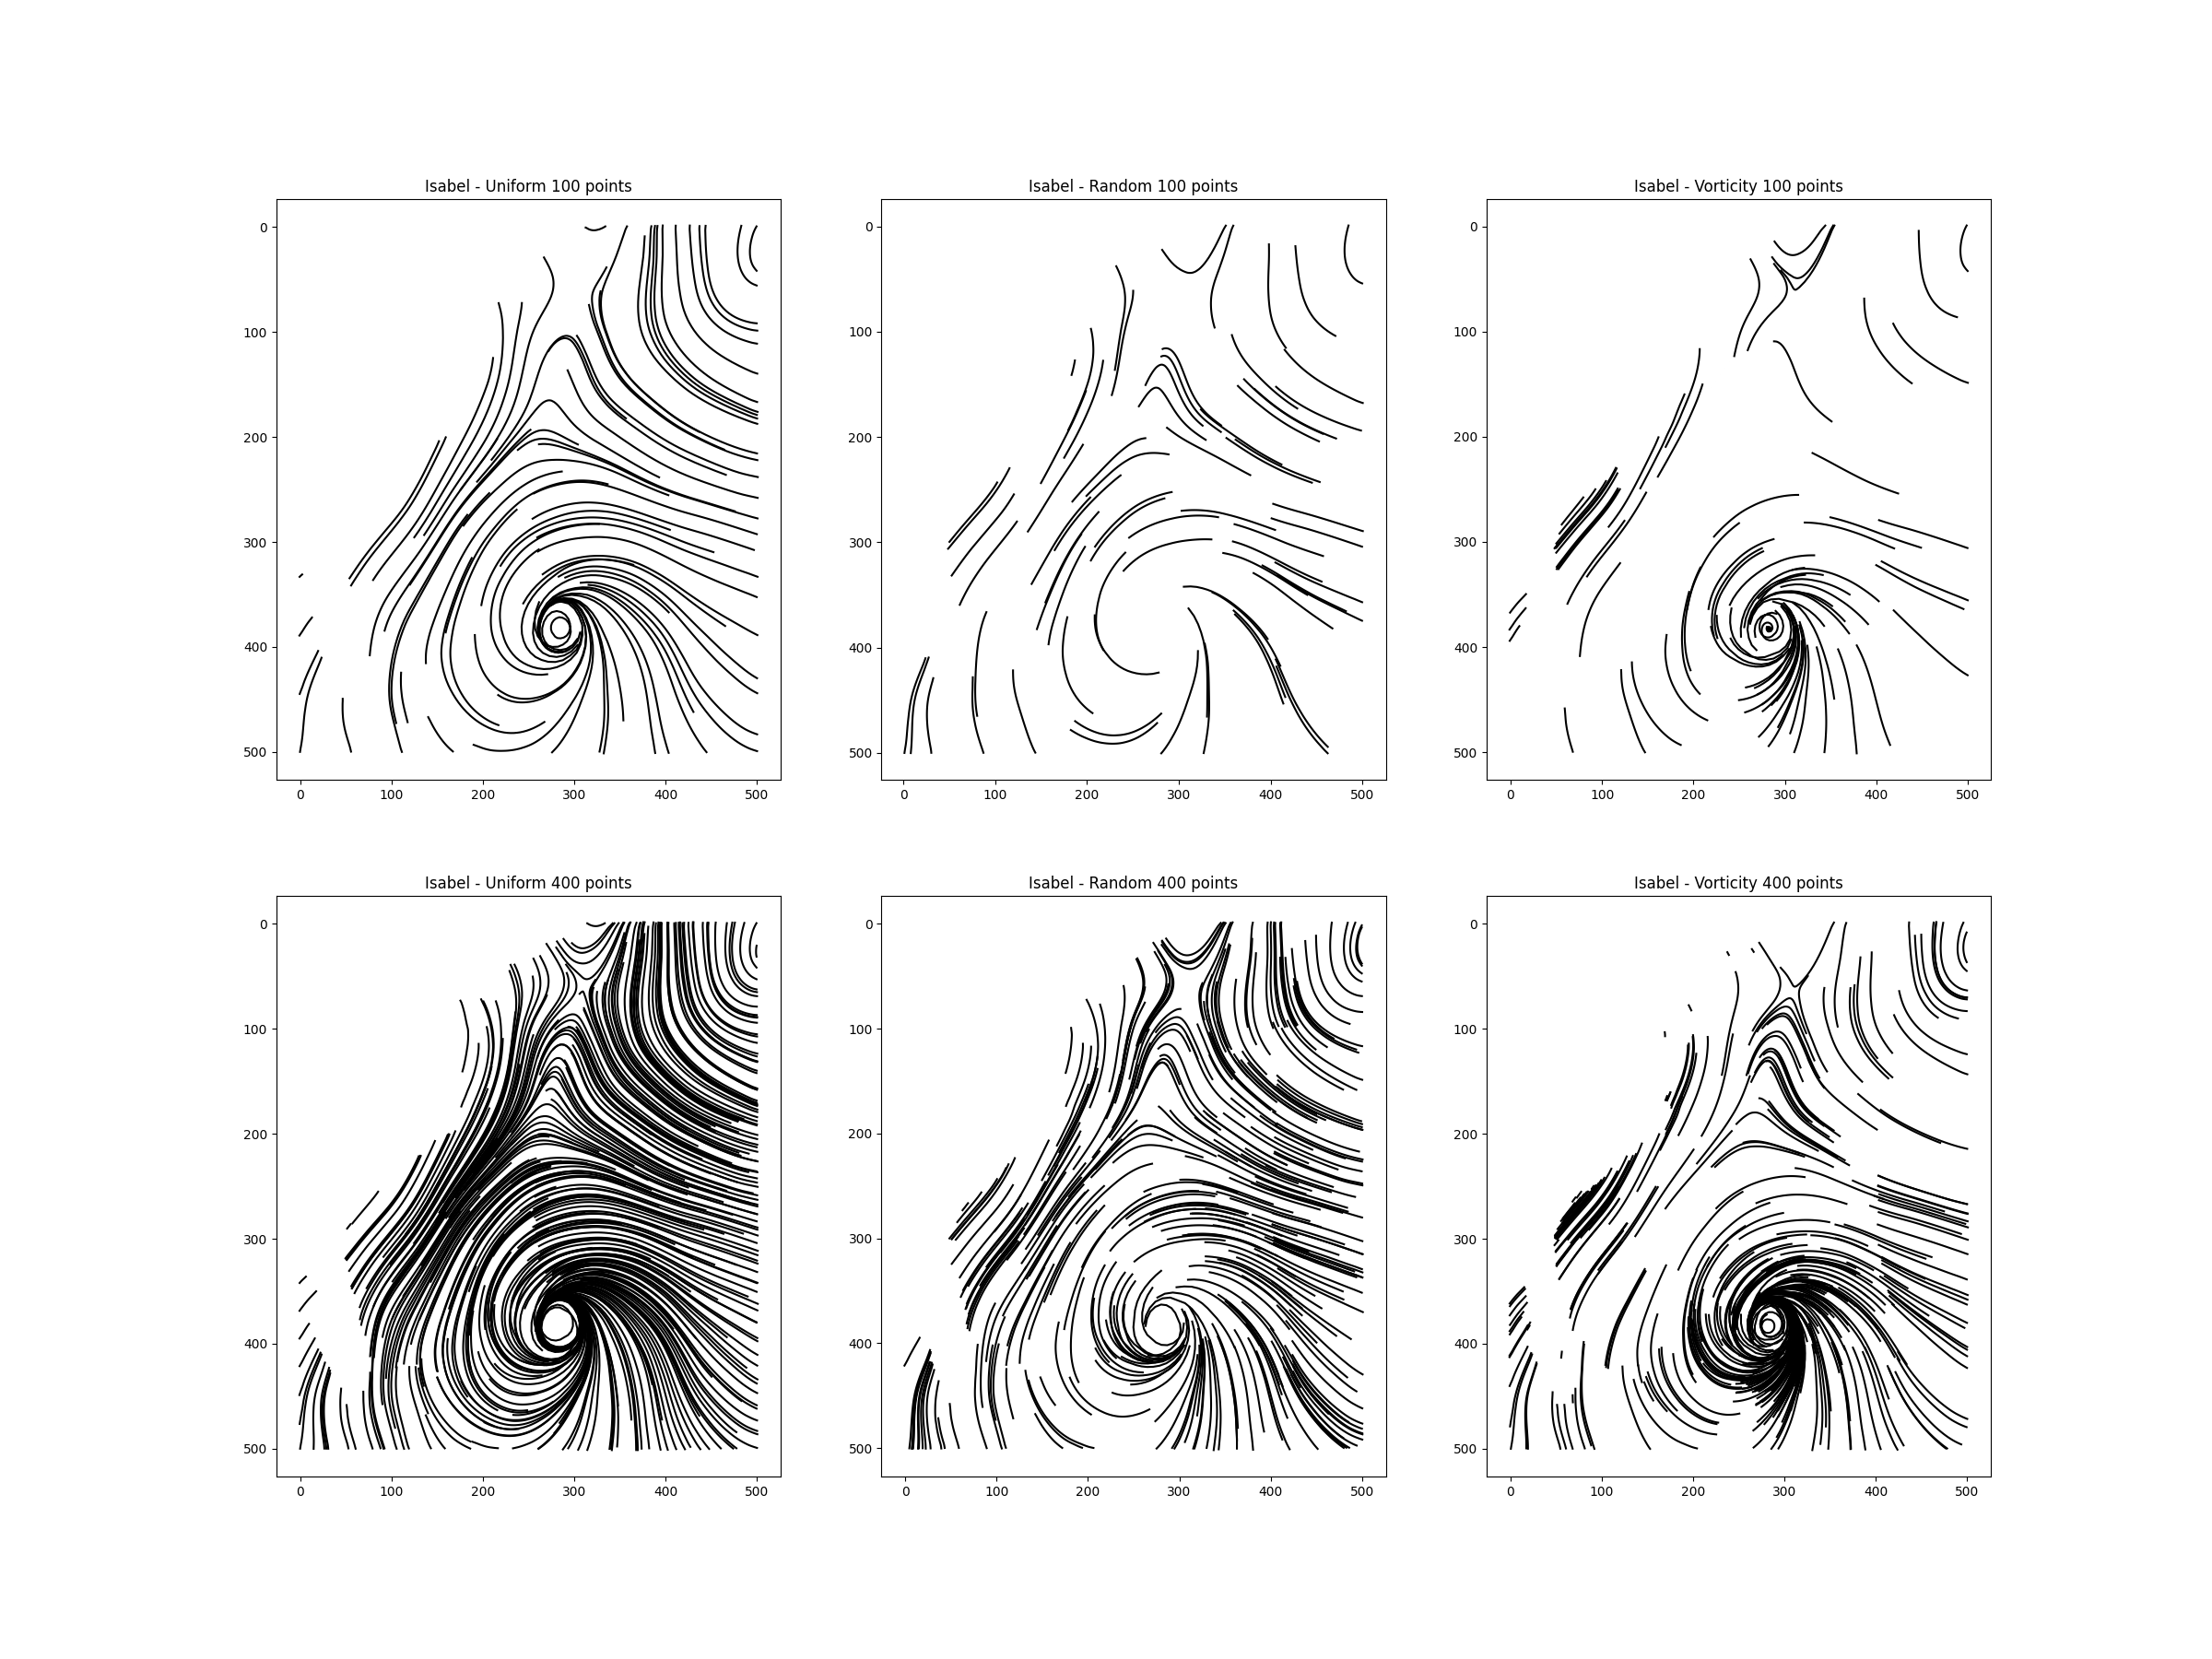
\includegraphics[width=18cm]{../output/isabel_seed_density.png}}
\caption{Comparison of seeding densities on the Isabel data}
\end{figure}

The two types of integrator also shows some differences. They have both been visualised
using the uniform seeding method to minimise the difference in visuals from the seed
points being different with random seeding. In the slower parts of the fields, the
differences are not really noticeable. Near areas of high curvature however, like
the swirl in the middle of Metsim or the storm in Isabel, the difference becomes
quite noticeable.

In the eye of the storm, the forward Euler integrator with a step of $dx = 1$ is
clearly struggling, drawing sharp lines that cross directly through the eye of
the storm leaving a large gap in the middle of it. Runge Kutta 4 fares better,
but is still clearly plagued by the hard turns in the field lines.

With a time step of $dx = 0.1$ both integrators create much better field lines.
The curves created by the RK4 integrator are noticeably smoother and more well behaved.
The forward euler integrator implementation used here also seems to have problems
with drawing the fields lines both ways, something that is yet to be resolved. The
difference in quality is still noticeable however, with the RK4 integrator creating
a nice circling around the eye of the storm and nicer curves near the saddle in the
north of the Isabel data.

\begin{figure}
\makebox[\textwidth][c]{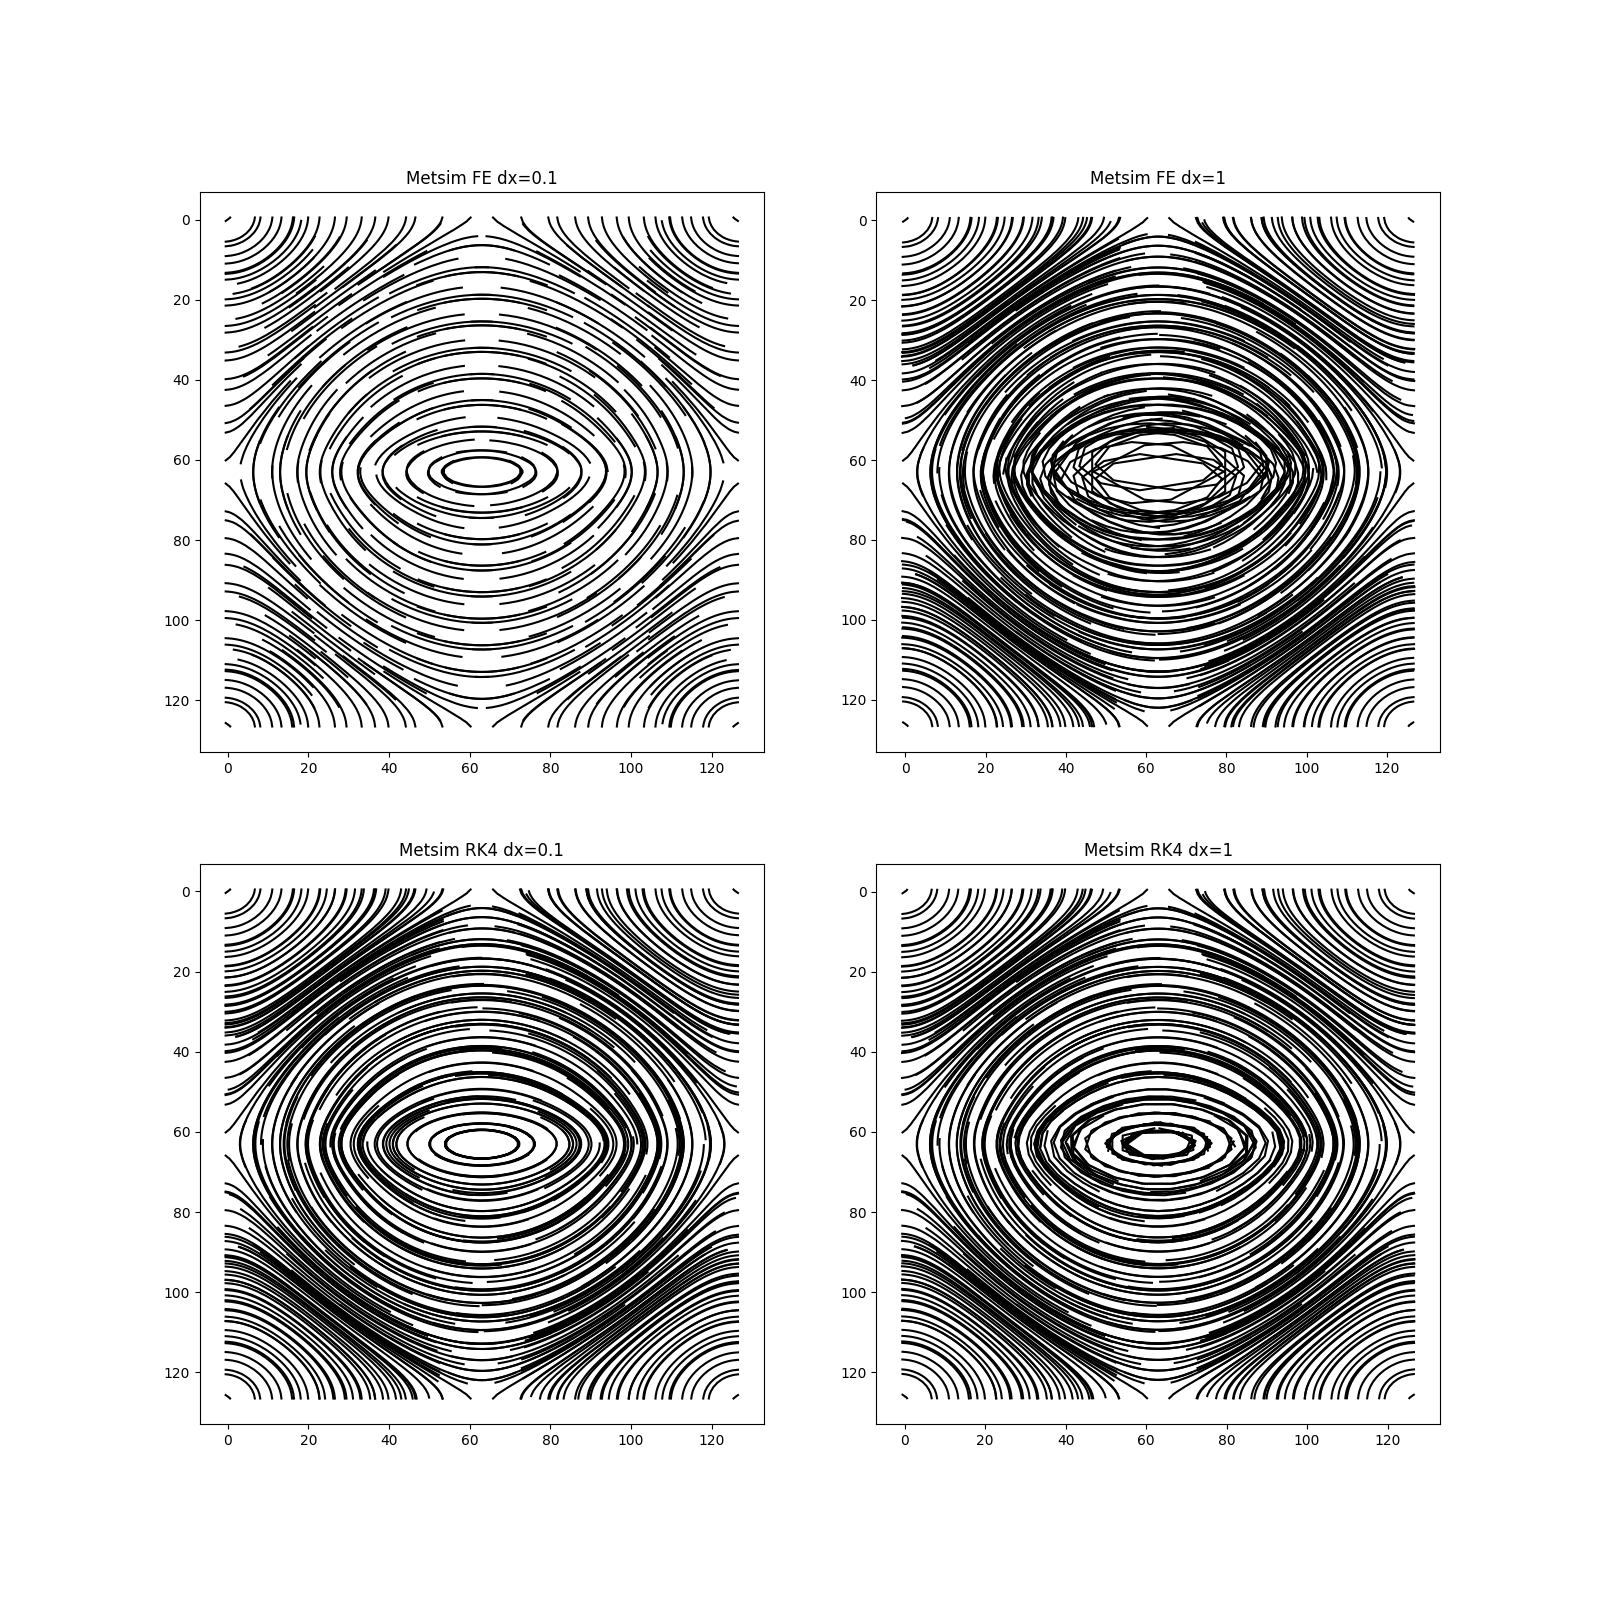
\includegraphics[width=18cm]{../output/metsim_integrator_dx.png}}
\caption{Comparison of integrators Forward Euler and Runge Kutta 4 with Metsim data}
\end{figure}

\begin{figure}
\makebox[\textwidth][c]{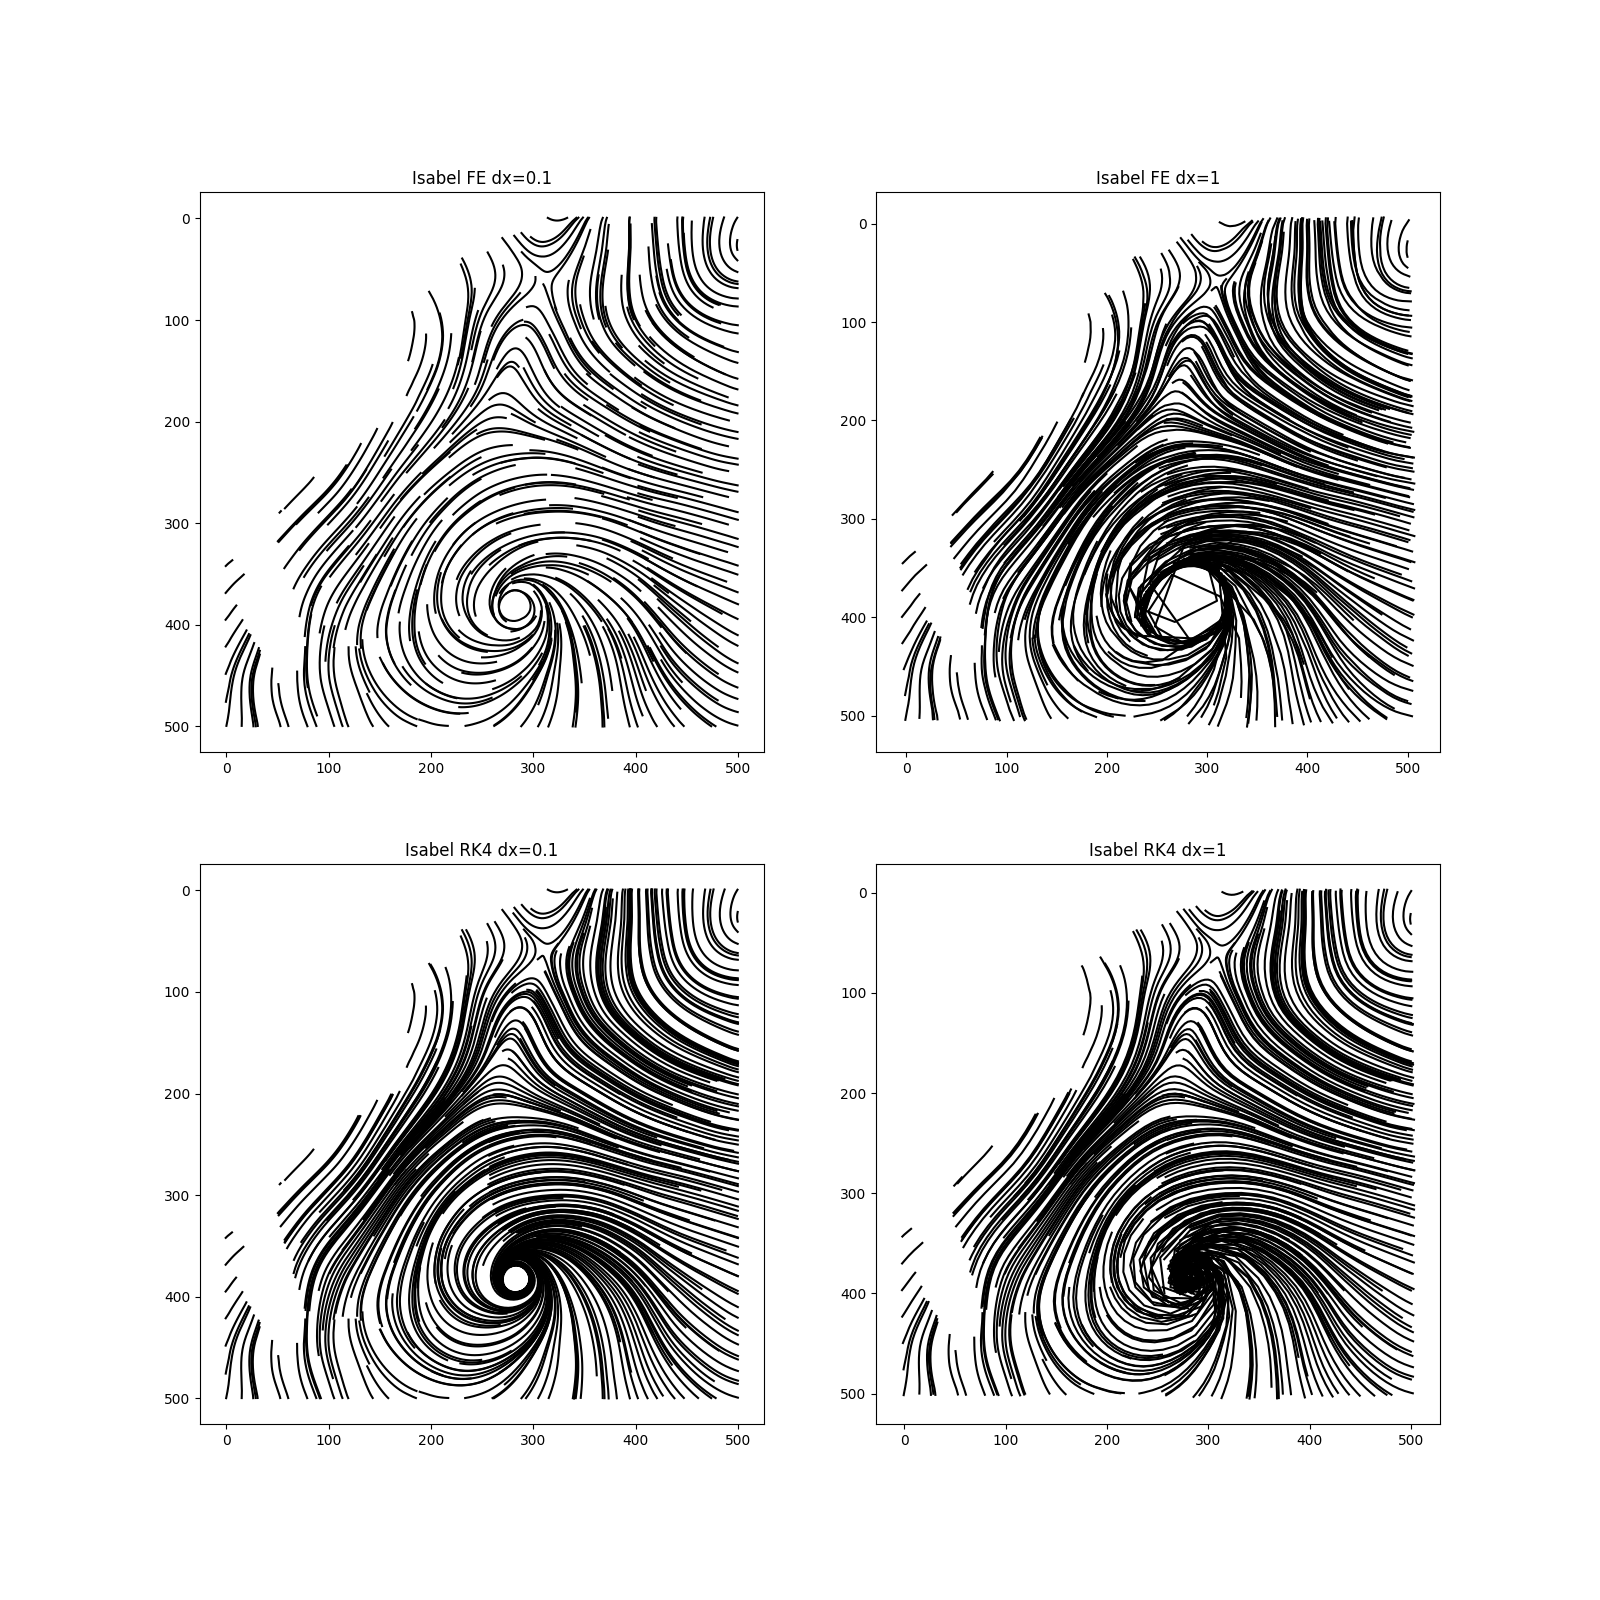
\includegraphics[width=18cm]{../output/isabel_integrator_dx.png}}
\caption{Comparison of integrators Forward Euler and Runge Kutta 4 with Isabel data}
\end{figure}

For the two different line lengths tested, some clear differences emerge. The shorter
lines give a nice and clear, though less cohesive, picture of the flow than their
longer counterpart. The less cluttered result from the short field lines gives
a result more reminiscent of a clearer version of a glyph visualisation, without the
direction. Still a clear image of the flow, but less insightful than the longer lines.

\begin{figure}
\makebox[\textwidth][c]{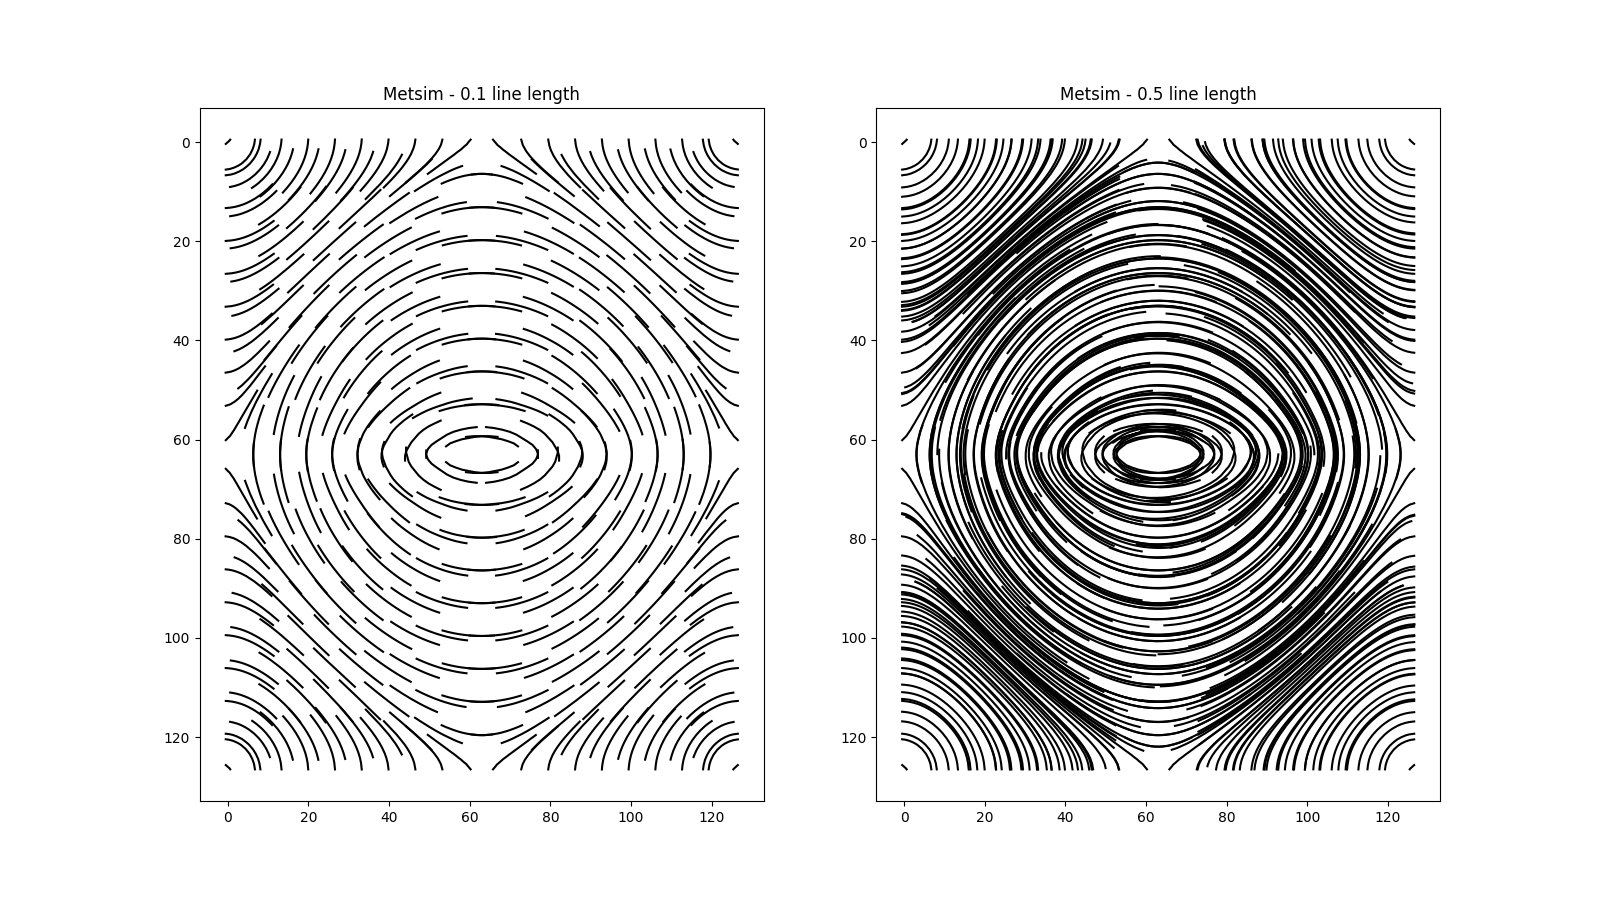
\includegraphics[width=18cm]{../output/metsim_line_length.png}}
\caption{Comparison of field line lengths with Metsim data}
\end{figure}

\begin{figure}
\makebox[\textwidth][c]{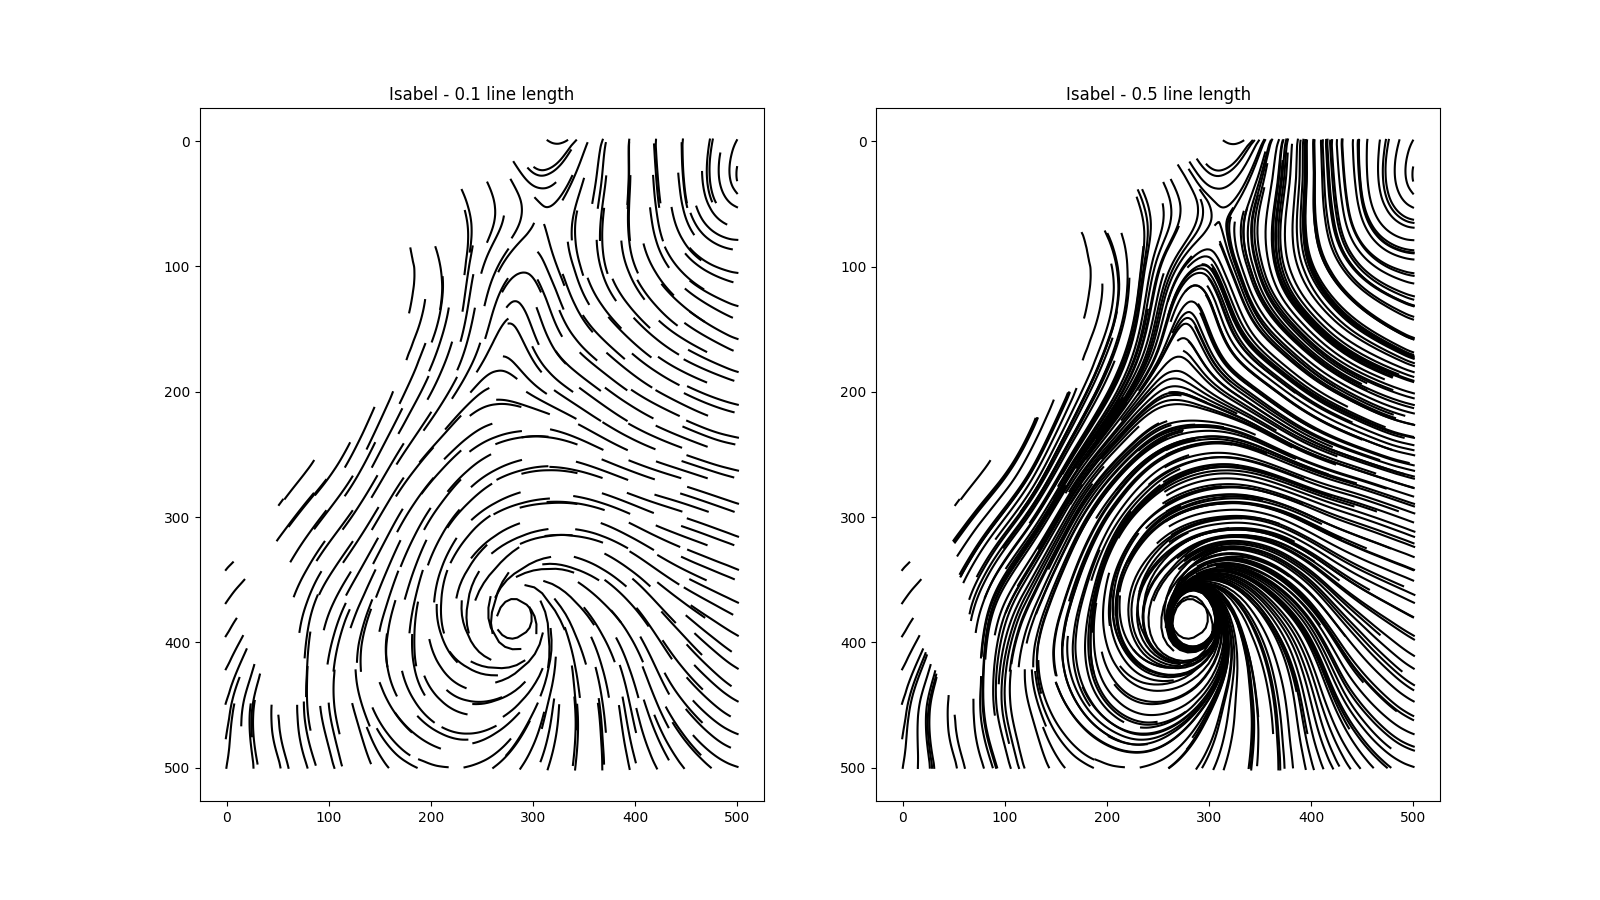
\includegraphics[width=18cm]{../output/isabel_line_length.png}}
\caption{Comparison of field line lengths with Isabel data}
\end{figure}

\section{Line Integral Convolution}
\subsection{Theory}
Line integral convolution is a method for creating textures that represent a vector
fields movement by combining field lines with a convolution along said field lines
on a texture, usually a noise texture. A white noise texture is a common type to
use for this, but other images may be used to.

To create the image, a seed point is created for every pixel in the input image.
A field line in accordance with the input vector field, scaled to match the image,
is then drawn to a pre determined length with equally spaced points. A convolution
kernel is applied, smoothing the colour values along the field line, before summing
and normalizing. The result of this becomes the colour for this pixel in the resulting
output image. The colour of a pixel $p$ is given mathematically as
$$ I(p) = \int_{-L}^{L} f(s) T(\sigma_p(s)) ds$$
where $\sigma_p$ is the field line originating at $p$, $T$ is the input texture,
$f$ is the convolution kernel and $L$ is the length of the field line in either
direction from its start.

\subsection{Implementation}
The implementation used in this project is a rather simple one, using the same
field line integrator from the geometric visualisations with options for both
forward Euler and Runge Kutta 4.

The LIC implementation first generates a noise texture which matches the dimensions
of the vector field. Every single pixel in this texture is used as a seed point for
generating a field line. Field lines are calculated to a specified length given as
a proportion of the total image width, before
the sample from the noise texture at every point of the field line is collected. An
average is taken of the values as a combination convolution and normalisation, and
this is given as the final colour value for that pixel.

Quite a few improvements could be made to this implementation, starting with a better
and more granular convolution kernel. Using the average is smearing out the lines,
but does still result in a final image with visible flows. Optimisation is also something
that is sorely needed, as performance is far from optimal. For quite short line lengths
the performance is not too bad, but unexpected patterns and waves start emerging in the
texture for these, as can been seen with the LIC of line length $0.2$. The choice
of integrator also noticeably effected performance, with forward Euler being quite
a lot faster, and without as much impact on the final result at could be seen in
the geometric approach. Some sharpening may also be a welcome post processing step.

\begin{figure}
\makebox[\textwidth][c]{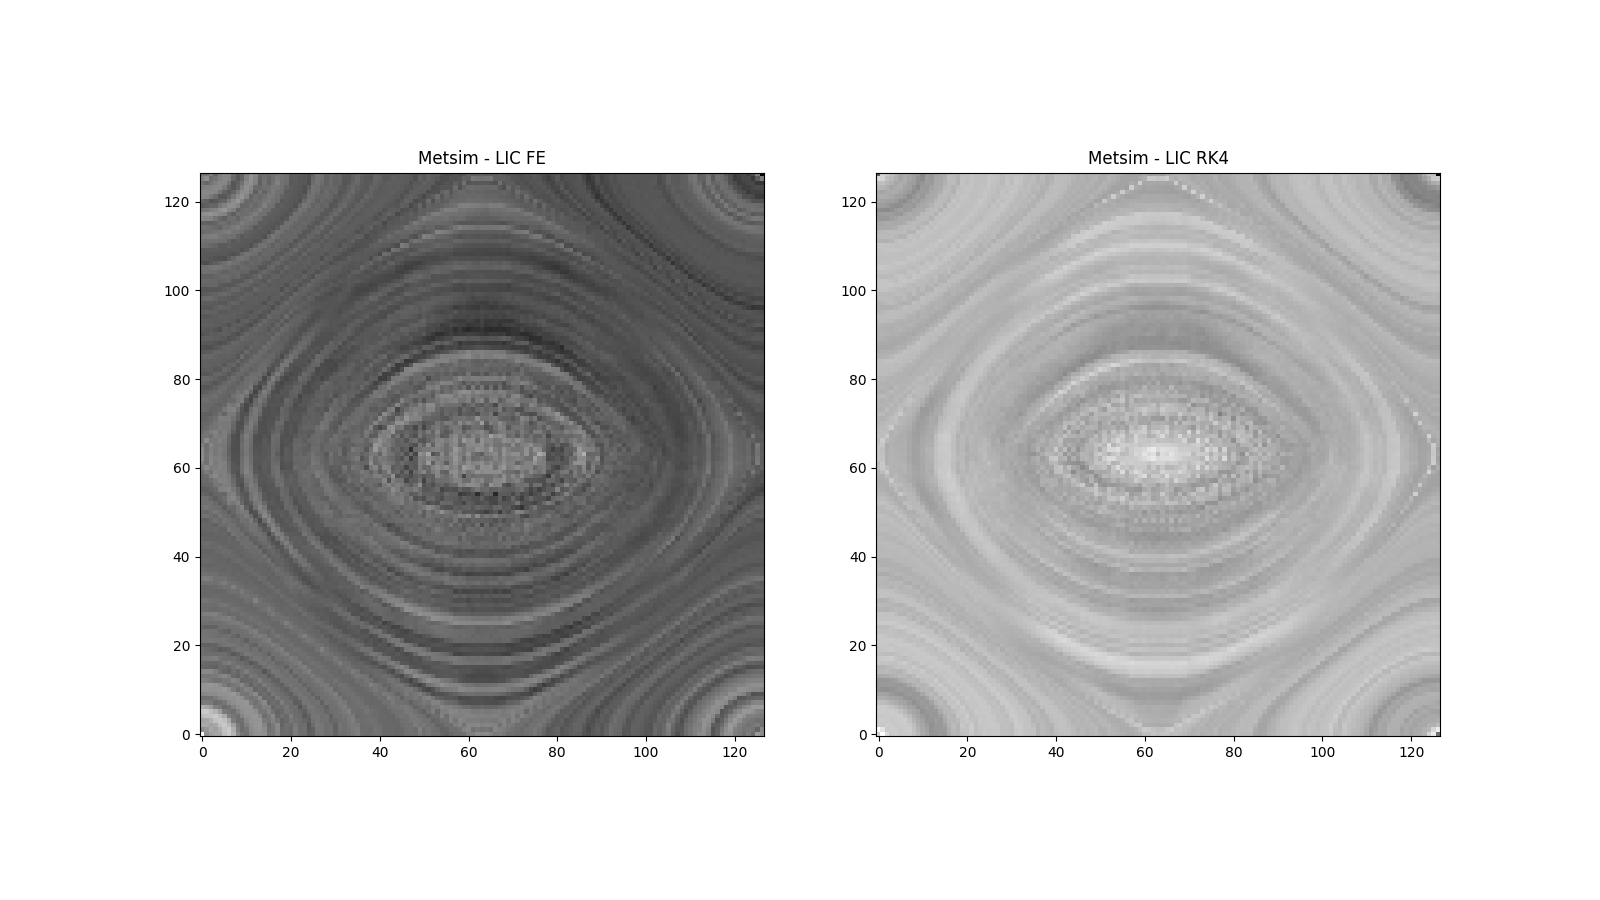
\includegraphics[width=18cm]{../output/metsim_lic_integrator.png}}
\caption{Comparison of integrators for LIC: Forward Euler and Runge Kutta 4 with Metsim data}
\end{figure}

\begin{figure}
\makebox[\textwidth][c]{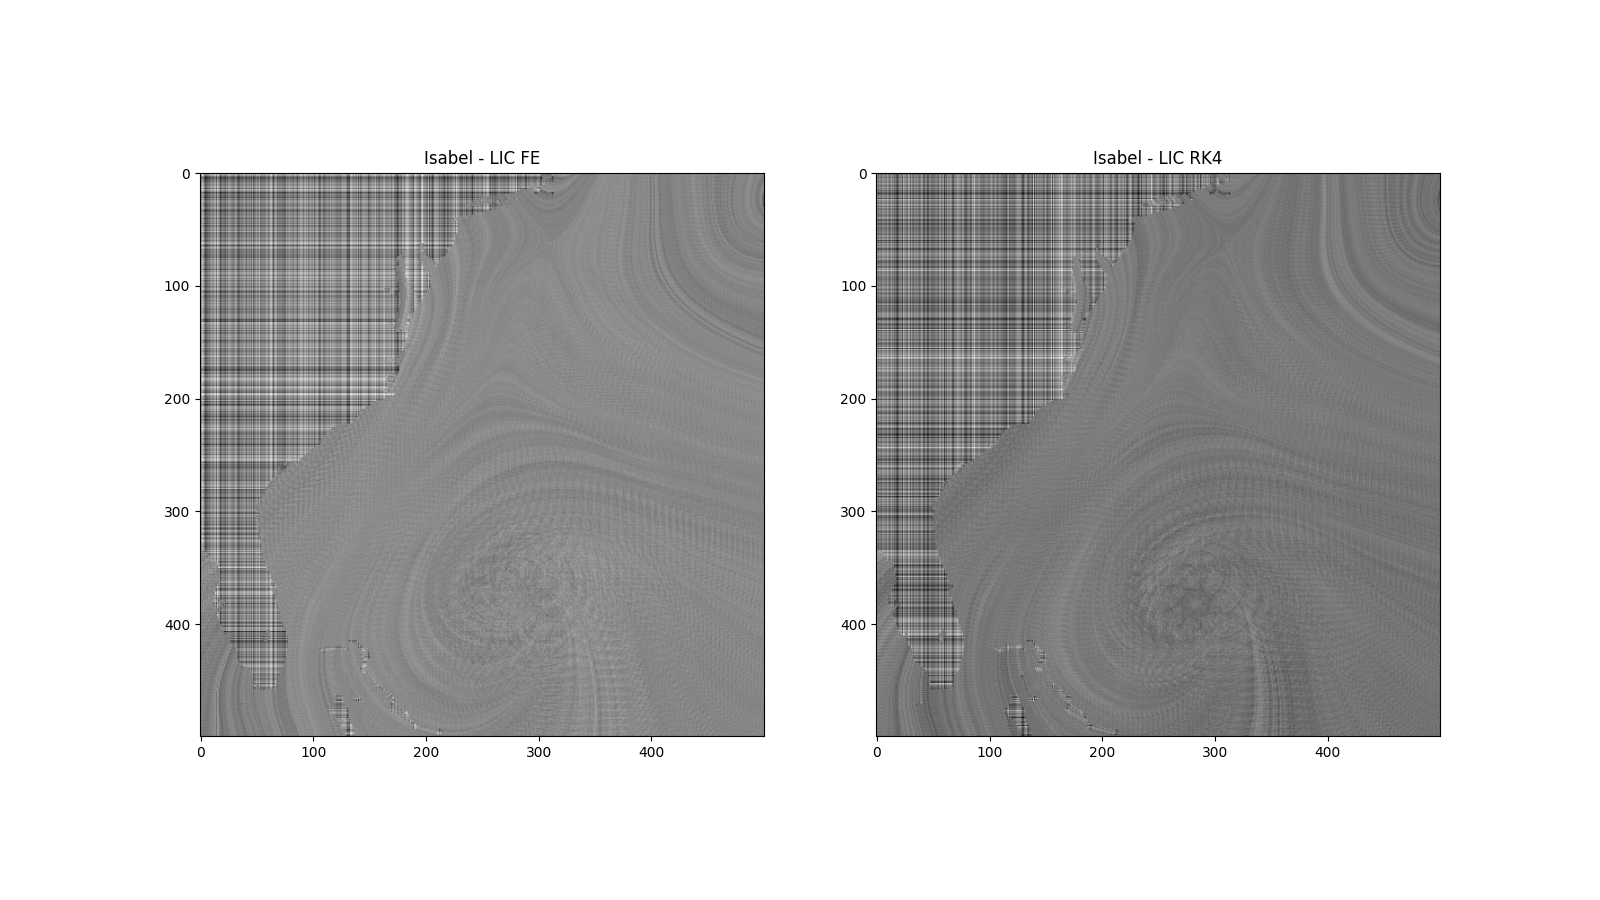
\includegraphics[width=18cm]{../output/isabel_lic_integrator.png}}
\caption{Comparison of integrators for LIC: Forward Euler and Runge Kutta 4 with Isabel data}
\end{figure}

In the plots for the line integral convolution, the plots that compare the two integrators
tested show very little difference between the two results. The flow pattern being
convoluted and summed into every field line only representing a single pixel seems
to drown out the impact small deviations have on the result, unlike in the field lines.
The field lines being drawn directly mean that small changes in the lines path change
very directly how the resulting visualisation ends up. Field lines being inaccurate mean
they may cross unnecessarily, or lay very close to each other, both creating more clutter.

The LIC images are an elegant and simple way to give a very comprehensive insight into
the flow.

\begin{figure}
\makebox[\textwidth][c]{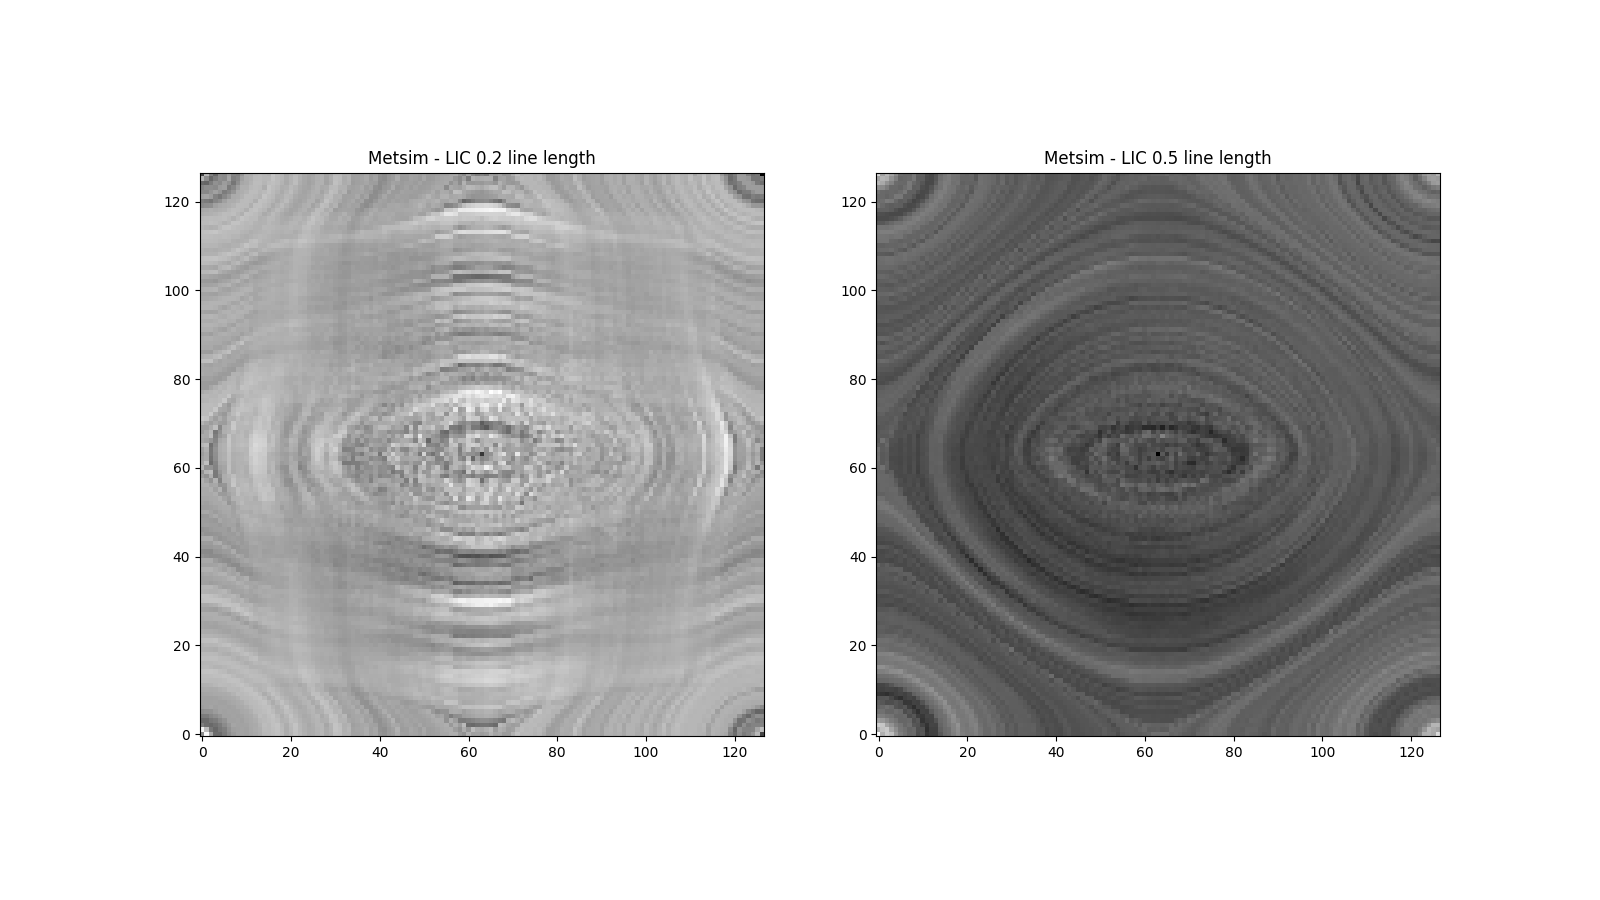
\includegraphics[width=18cm]{../output/metsim_lic_line_length.png}}
\caption{Comparison of LIC filter lengths: 0.2 vs 0.5}
\end{figure}

\begin{figure}
\makebox[\textwidth][c]{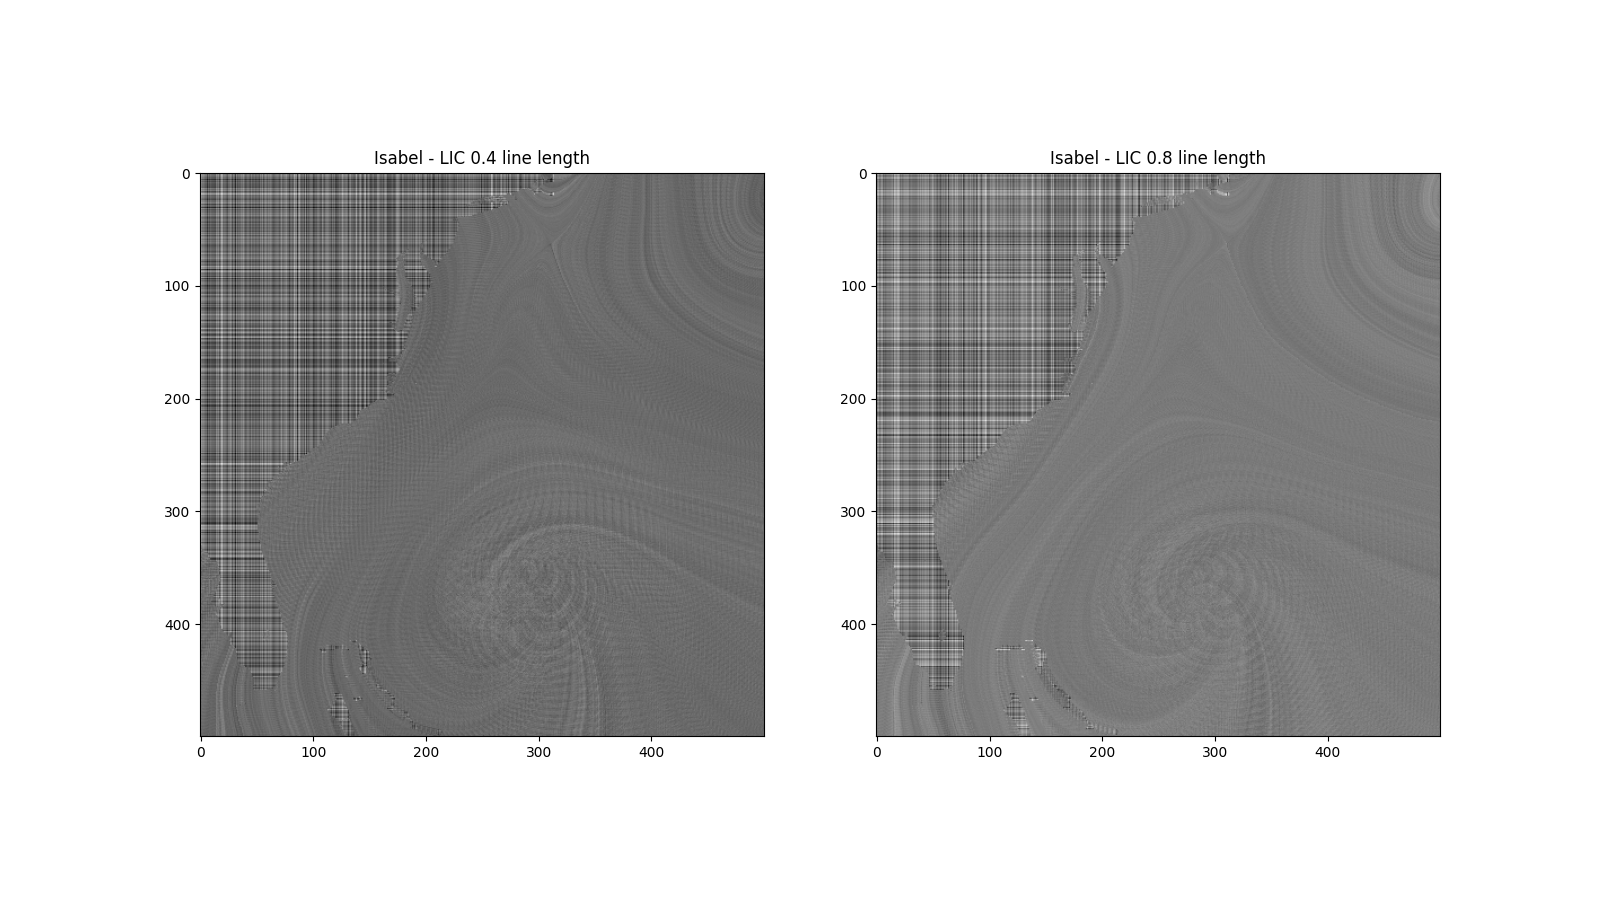
\includegraphics[width=18cm]{../output/isabel_lic_line_length.png}}
\caption{Comparison of LIC filter lengths: 0.4 vs 0.8}
\end{figure}

The filter core length has a very clear impact on the LIC result, both in result
and computational time. The code used here has shown itself to be subpar when it comes to efficiency
highlights this very well. The longer field lines LIC images have taken upwards of hours to compute,
with the fastest still taking almost a minute. The shorter line lengths seem to get artifacts,
in the final visualisation. For line lengths like the $0.2$ and $0.3$ for the Metsim and the $0.05$
for Isabel, the resulting image has smeared section. For the Metsim data, this looks like an overlayed
alternating flow, but when looking at the Isabel data with the short lines, these seem to be smears
in the direction of the grid. The same pattern can be seen in the areas of no flow in the Isabel set,
with the only thing remaining being the grid pattern.

\section{Comparison of methods}
The two methods give very similar representations of the flow, creating lines along
the flow, although in very different ways. The geometric field lines give a very high
clarity of the flow. When covering the field adequately, but not too densely, they give a good look
at the flow characteristic and points or regions of interest.

The field lines give a high degree of customisability to how much is shown. This effects both the
computational load of drawing the field lines, but also what to highlight in the flow. As can be
seen with the vorticity based seeding, regions of interest can have more seeds for field lines,
meaning higher clarity where necessary. This may however also be a problem, as rapidly changing
flows will require many field lines, making the areas cluttered, or leaving gaps in other parts of
the field.

The LIC however gives a much greater degree of coverage for the field, and can
create more visually pleasing imagery, especially seeing as the LIC images can be
created in higher resolution than the vector field it self is defined in. The LIC
visualisation requires a field line to be computed for every pixel in the input image, which
for sub optimal implementations is incredibly computationally costly. It does mean that every
single pixel of the final output has taken the flow through it into account though.

The better coverage of LIC seems to give it a clear advantage for more complicated
patterns of flow. The high clarity of the field lines however seems to give them a greater
degree of precision in flows that do not change characteristics rapidly. Both these
visualisation techniques are invaluable tools to have at ones side, and work great
for different types of flow, with some overlap.

To summarise: field lines are computationally cheap, and can be drawn where the flow is interesting
to highlight the important areas. It may however miss important parts of the flow if not fine tuned.
LIC on the other hand is expensive, but misses no part of the flow and thus requires little tuning
to give a good result.


\section{Further work}
More and better strategies for seeding have been developed over the years, and
methods that combine the drawing of the field lines with creating new seed points
seem like a great way to minimise clutter, give greater clarity, and minimise waste
of compute time in drawing the field lines. This, along side more optimised code
either through Numpy vectorisation or jit-compiling, are clear improvements to the
geometric visualisation done here.

On the LIC front there are still lots of improvements to be made. The optimisation
of the field line drawing is a good first step, but a better understanding and use
of proper convolution kernels, as well as contrast increasing post processing
could create less smeared results. The current results are very grey, with little
white and black showing through. The flow patterns are visible in the final result,
but not as clearly as they could be.

The aliasing patterns showing up are also a problem, presumably one stemming from the
lack of proper convolution. The saddle point in the Isabel data still clearly show up,
but the eye of the storm is less clearly visible, especially when compared to the geometric
field lines.

\section{Conclusion}
The two methods discussed in this report are excellent tools for visualising
vector field data in different ways, and with clear advantages in their own ways.
They respond differently to different ways of minimising compute time, like the field
lines being sensitive to the integrator while the LIC is sensitive to line length.
Both of these methods are certainly ones that will come in handy in future work.

\end{document}
